\documentclass[aps,superscriptaddress, notitlepage,longbibliography]{revtex4-1}
\usepackage{hyperref}
\usepackage{amsmath}
\usepackage{physics}
\usepackage[pdftex]{graphicx}
\usepackage{xcolor}
\setlength {\marginparwidth }{2cm}
\hypersetup{
    colorlinks,
    citecolor=blue,
    filecolor=black,
    linkcolor=red,
    urlcolor=blue
}

\newcommand{\comment}[1]{{\color{blue}#1}}
\newcommand{\edit}[1]{{\color{purple}#1}}
\newcommand{\del}[1]{{\color{red}\st{#1}}}
\newcommand{\beginsupplement}{%
        \setcounter{table}{0}
        \renewcommand{\thetable}{S\arabic{table}}%
        \setcounter{figure}{0}
        \renewcommand{\thefigure}{S\arabic{figure}}%
     }
% Standardize command font styles and environments
\newcommand{\doccmd}[1]{\texttt{\textbackslash#1}}% command name -- adds backslash automatically
\newcommand{\docopt}[1]{\ensuremath{\langle}\textrm{\textit{#1}}\ensuremath{\rangle}}% optional command argument
\newcommand{\docarg}[1]{\textrm{\textit{#1}}}% (required) command argument
\newcommand{\docenv}[1]{\textsf{#1}}% environment name
\newcommand{\docpkg}[1]{\texttt{#1}}% package name
\newcommand{\doccls}[1]{\texttt{#1}}% document class name
\newcommand{\docclsopt}[1]{\texttt{#1}}% document class option name
\newenvironment{docspec}{\begin{quote}\noindent}{\end{quote}}% command specification environment


\DeclareMathOperator*{\argmax}{arg\,max}
\DeclareMathOperator*{\argmin}{arg\,min}

\definecolor{pastel_green}{rgb}{0.18,0.65,0.34}
\newcommand{\CHW}[1]{\textcolor{pastel_green}{#1}}
%% OPTIONAL MACRO DEFINITIONS
\def\s{\sigma}


\def \M{\mathcal{M}}  
\def \P{\mathrm{P}}
\def \E{\mathbb{E}}


\def \mcl{\mathcal}
\def \mbb{\mathbb}
\def \mbf{\mathbf}



\def\bd{\boldsymbol}
\def\sm{\setminus}
\def\tb{\textbf}

\def\CH{\cal{H}} 

\def\<{\langle}
\def\>{\rangle}

\def\thet{{\theta}^{(t)}}
\def\thetp{{\theta}^{(t+1)}}
\def\thets{{\theta}^{(t)\star}}


\def\be{\begin{equation}} 
\def\ee{\end{equation}}
\newcommand \bea {\begin{eqnarray}} 
\newcommand \eea {\end{eqnarray}} 
\newcommand \sign {\hbox{sign}} 
\newcommand{\nn} {\nonumber}
\newcommand{\mbbE} {\mathbb{E}}
\begin{document}

\title{scTOP: physics-inspired order parameters for cellular identification and visualization}

\author{Maria Yampolskaya}
\email{mariay@bu.edu}
\affiliation{Department of Physics, Boston University, Boston, MA 02215, USA}
\author{Michael J Herriges}
\affiliation{Center for Regenerative Medicine of Boston University and Boston Medical Center, Boston, MA, USA}
\affiliation{The Pulmonary Center and Department of Medicine, Boston University School of Medicine, Boston, MA, USA}
\author{Laertis Ikonomou}
\affiliation{Department of Oral Biology. University at Buffalo, The State University of New York, Buffalo, NY, USA}
\affiliation{Division of Pulmonary, Critical Care and Sleep Medicine, Department of Medicine, University at Buffalo, The State University of New York, Buffalo, NY, USA}
\author{Darrell N Kotton}
\affiliation{Center for Regenerative Medicine of Boston University and Boston Medical Center, Boston, MA, USA}
\affiliation{The Pulmonary Center and Department of Medicine, Boston University School of Medicine, Boston, MA, USA}
\author{Pankaj Mehta}
\email{pankajm@bu.edu}
\affiliation{Department of Physics, Boston University, Boston, MA 02215, USA}
\affiliation{Center for Regenerative Medicine of Boston University and Boston Medical Center, Boston, MA, USA}
\affiliation{Faculty of Computing and Data Science, Boston University, Boston, MA 02215, USA}
\affiliation{Biological Design Center, Boston University, Boston, MA 02215, USA}

\maketitle

\section*{Supplementary Information}
\beginsupplement

\subsection{Interpreting scTOP scores}\label{interpretation}
In theory, the attractor-network order parameters we have adapted for gene expression data range between negative one and positive one. An attractor state order parameter with a value of positive one means the system is perfectly aligned with that particular attractor state, and negative one means it is the exact opposite of that attractor state. Zero means that it is neither correlated nor anti-correlated with that attractor state. 

In practice, scTOP scores generally do not reach positive one. scRNA-seq data contains significant numbers of dropouts, and these zeroes decrease the magnitude of the scTOP score. When an aggregate score is taken, the effect of dropouts is decreased and the scTOP score increases. This is important to keep in mind when interpreting scTOP scores; any score above 0.1 is notable, and since the data is so noisy even the best-case score may be well below 1. It's helpful to have a control population to compare with, to have a measure of the range of best-case scTOP scores. This is also why it's best to compare distributions of scores rather than scores for individual cells, since noise plays a non-negligible role.

scTOP scores are rarely negative. Negative values for scTOP scores correspond to cases where the sample gene expression profile is the opposite of the reference profile. For example, a score of -1 would indicate that all the genes which are highly-expressed in the reference are lowly-expressed in the sample, and vice versa. There are cases where the scores are low, negative values, indicating that the sample does not align well with the reference and that some genes which are highly- (lowly-) expressed in the reference are lowly- (highly-) expressed in the sample. From the data, it appears that it’s unlikely for gene networks to contain cell types which are opposites of one another. One possible reason is that some genes, like housekeeping genes, are similarly expressed across all cell types. Also, it’s possible that cells which expressed the exact opposite genes of any given cell type would not be able to survive.


\subsection{Comparison to other linear methods}
scTOP is mathematically and conceptually distinct from other linear methods such as Principal Component Analysis (PCA). PCA takes input data and finds the vectors in feature space along which the most sample-to-sample variation occurs. PCA is unsupervised and assumes nothing is known about the input data. The principal components need to be examined to determine their biological relevance. The major difference with scTOP is that scTOP takes input data and a reference basis of known cell types. The input data is decomposed onto the vectors defined by the reference basis instead of vectors corresponding to the most sample-to-sample variation. With scTOP, the resulting decomposition has a direct interpretation: alignment with each of the known cell types within the reference basis. It’s not possible to find the decomposition onto known cell types with PCA, because PCA doesn’t have the extra information about pre-defined cell type expression profiles. 

To summarize, scTOP and PCA both transform the sample data to a different coordinate system, but there are major differences between the spaces that these methods project onto. The following table breaks down the differences between these spaces.

\begin{tabular}{ |p{3in}|p{3in}|} 
 \hline
 scTOP space & PCA space\\ 
 \hline
 \hline
 Defined by an input reference basis of known cell types & Calculated by PCA by finding the orthogonal vectors (principal components) that best explain the variation in data  \\ 
 \hline
 Can be non-orthogonal (e.g. can have highly-correlated cell types) & Orthogonal by definition  \\ 
 \hline
 Dimensions have clear biological interpretation: alignment with cell types & Dimensions need to be closely analyzed to be interpreted \\
 \hline
\end{tabular}

\subsection{Preprocessing} \label{preprocessing}
The raw scRNA-seq count data for each dataset was downloaded as a matrix of mRNA counts corresponding to genes and cells. An example of such a matrix is shown in step 0 of figure \ref{FIG:supp1}, where each row is a different gene, and each column is a different cell. Throughout this figure, the histogram to the right of each step shows the distribution of entry values for the first column (cell) in the matrix, and the histogram below the step shows the distribution of entry values for the second row (gene Rpl7) of the matrix. The histograms are presented as examples of how the distributions (for each cell and gene) of gene expressions change as the data is preprocessed.

In the first step of preprocessing, each cell is normalized independently. This step is taken because scRNA-seq generally measures relative rather than absolute expression levels within a cell. In order to facilitate the comparison of cells across sequencing conditions, we transform the normalized RNA counts into quantities that are centered around the mean expression level. Z-scores are exactly such a quantity; they measure the number of standard deviations away from the mean. To calculate the z-scores after step 1, we convert the normalized gene expressions into percentiles by ranking each gene in a given cell from lowest to highest, then dividing by the number of genes (plus one so that the highest rank is not assigned the 100th percentile). For example, if a cell has 1000 genes sampled and Rpl7 is the highest-expressing gene, it will be given rank 1000 and labeled as the 99th percentile. If two or more genes are tied for rank, as is the case for zero-values, they are assigned the average of the ranks they would have been assigned if they were not tied (see rankdata function from the Python package Scipy). To convert from percentiles to z-scores, we assumed a normal distribution with mean 0 and standard deviation 1 and applied the corresponding quantile function.

\begin{figure}
	\centering
		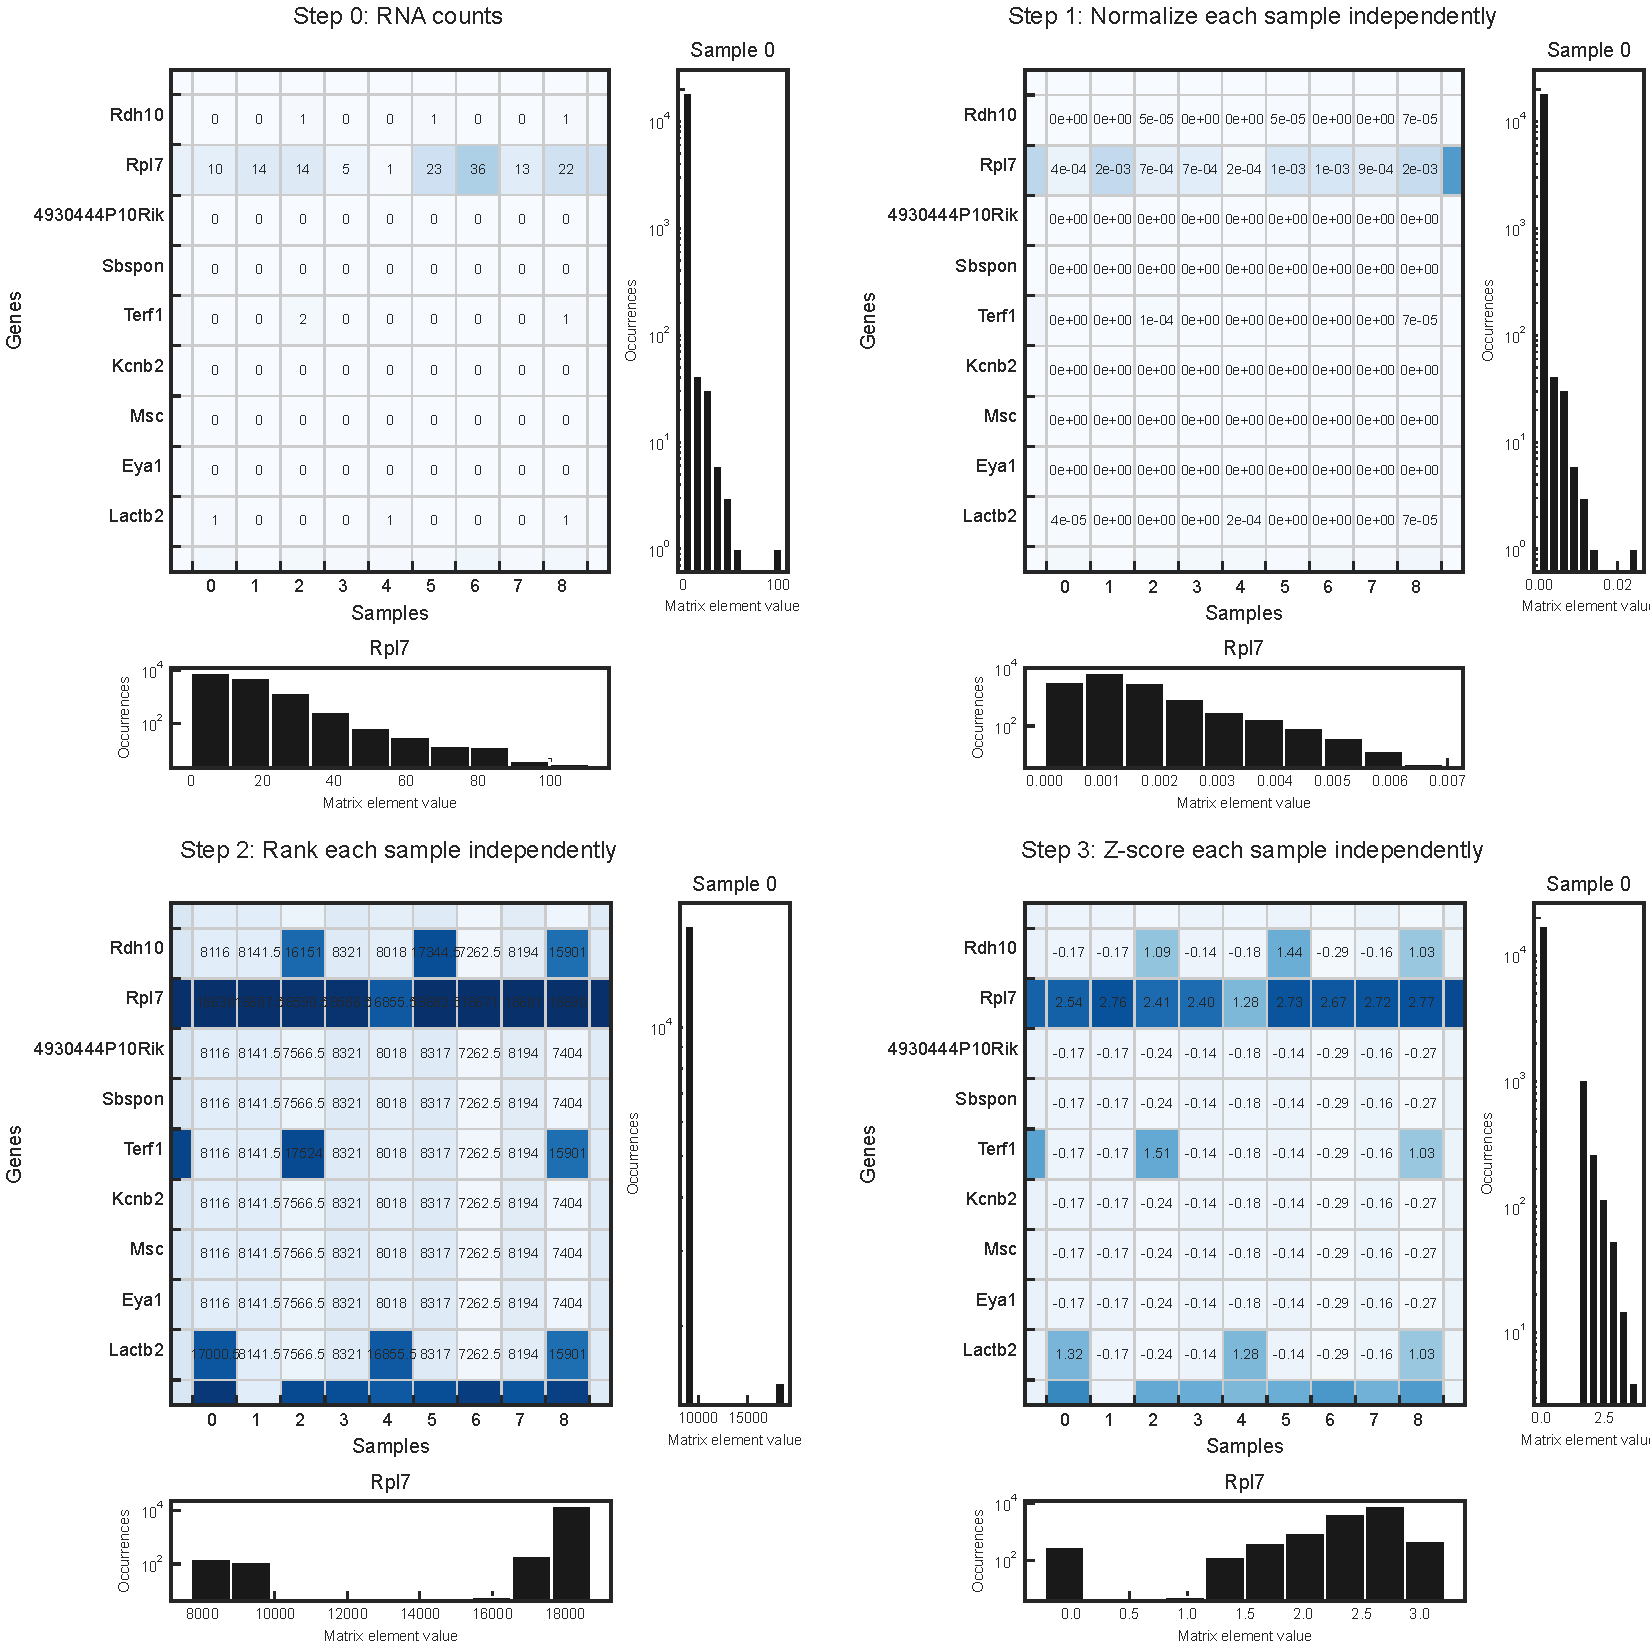
\includegraphics[scale=0.6]{figs/fig1a supplement.pdf}
	\caption{Data distributions at each preprocessing step. Step 0 shows the original RNA count matrix before preprocessing, where each entry corresponds to the number of RNA detected for a particular gene in a particular cell. The rows of each matrix correspond to genes, and the columns correspond to cells. The histograms to the right of each matrix show the distribution of an example cell, while the histograms below each matrix show the distribution of an example gene. Step 1 of preprocessing is to normalize each cell. Steps 2 and 3 convert the normalized gene expressions to z-scores. Step 2 ranks the genes in each cell according to magnitude and converts the rank into a percentile. Step 3 uses a quantile function, assuming a normal distribution with mean zero and standard deviation one, to convert from percentiles to z-scores.}
	\label{FIG:supp1}
\end{figure}

\subsubsection{Preprocessing rationale} 

In order to mitigate batch effects, the preprocessing step in scTOP takes each cell and ranks each gene according to expression. These ranks are converted into percentiles, which are then transformed into z-scores assuming a normal distribution.
    
By ranking the genes before converting to z-scores, we are ignoring the absolute values of RNA counts and instead focusing on the relative values. Some sequencing platforms may measure many more counts than others; although we can't recover the unmeasured counts that are lost via dropouts, we can remove the effect of differences in counts by ranking. We assume that each cell contains similar numbers of mRNA and that the actual number of RNA doesn't matter as much as the relative expression of different genes. For example, the highest-expressed gene in one cell should be comparable to the highest-expressed gene in another cell, regardless of RNA count. Ignoring the absolute values of RNA counts reduces the differences caused by different scRNA-seq technologies and experiments, as shown in section \ref{batch effects section}.

The second preprocessing step is to convert the ranks to z-scores, assuming a normal distribution. This step results in a mean of zero and standard deviation of one. In data analysis, it is beneficial to standardize the data before comparing across datasets because this prevents a disproportionate bias towards features with large values. In the case of scTOP, having a mean of zero and a standard deviation of one is especially important because the underlying math relies on the dot product of two uncorrelated vectors to be zero and the magnitude of a vector to be one.

By ranking and z-scoring, we remove undue weighting of genes according to magnitude of expression, instead prioritizing the relative expression.

\subsection{Batch effects} \label{batch effects section}
scRNA-seq data produced using different sequencing platforms from different experiments may introduce variation in the form of batch effects. Because the pre-processing step in scTOP prioritizes the relative rather than absolute expression of genes, batch effects are mitigated.

Tran et al. \cite{tran2020benchmark} consolidated datasets from different experiments for the purposes of benchmarking various batch-effect correction methods. One of these is a dataset containing scRNA-seq human pancreatic data from five different sources \cite{baron2016single} \cite{muraro2016single} \cite{segerstolpe2016single} \cite{wang2016single} \cite{xin2016rna}, using various sequencing technologies. We used scTOP to analyze these datasets. Figure \ref{batch effects} illustrates that scTOP is not significantly affected by differences between batches. Because the Baron et al. dataset had the most cells per cell type, we used it to create a reference basis consisting of alpha, beta, ductal, acinar, delta, gamma, stellate, and endothelial gene expression profiles. We projected cells from the other four experiments onto the Baron reference basis. The top row shows kernel density estimate (KDE) plots for cells that match the reference cell type (e.g. alpha scores for alpha cells) with solid lines, and cells that do not match the reference type but have higher scores than the other non-matching types (e.g. alpha scores for beta cells) with dashed lines. The bottom row shows box-and-whisker plots for the cells that match the reference type.

Despite coming from different sources, the distributions of scores are similar. There is also a clear bimodal distribution for cells that match the reference type and cells that don't. This bimodality is a clear indication that batch effects don't cause misidentification.

According to Ziegenhain et al. \cite{ziegenhain2017comparative}, Smart-seq2 detects the most genes per cell when compared to other sequencing methods of that time. This decrease in dropouts may explain why the Segerstolpe data (which is the only experiment that used Smart-seq2) has slightly higher projections than the other datasets.

\begin{figure}
	\centering
    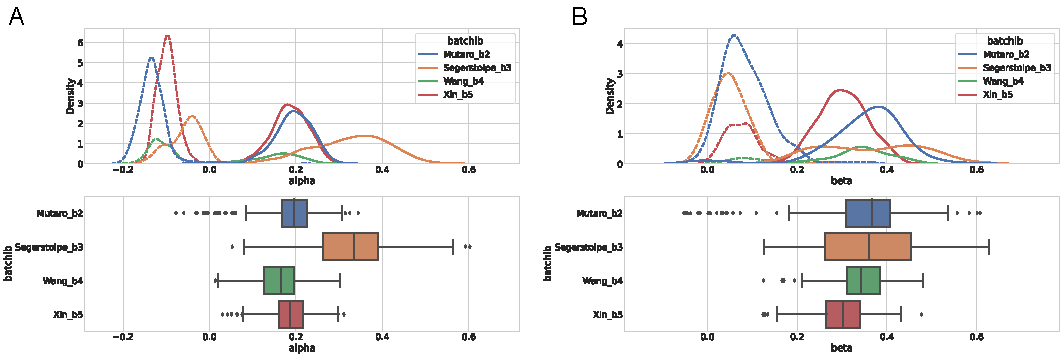
\includegraphics[scale=0.95]{figs/batch effects.pdf}
	\caption{Pancreatic data from different experiments using different scRNA-seq technologies. The reference basis uses data from Baron et al. \cite{baron2016single}, and the cells that are projected onto this basis are from Muraro et al. \cite{muraro2016single}, Segerstolpe et al. \cite{segerstolpe2016single}, Wang et al. \cite{wang2016single}, and Xin et al. \cite{xin2016rna} (A) Kernel density estimate (KDE) plot of alpha scTOP scores for alpha cells (solid) and beta cells (dashed), and a box-and-whisker plot of alpha scTOP scores for alpha cells. (B) KDE plot of beta scTOP scores for beta cells (solid) and delta cells (dashed), and a box-and-whisker plot of beta scTOP scores for beta cells. }
	\label{batch effects}
\end{figure}

\subsection{Reference basis construction}\label{basis construction}
Creating an appropriate reference basis is vital to the accuracy of scTOP. There are many existing scRNA-seq atlases, such as the Mouse Cell Atlas; using them with scTOP requires some amount of curation. For each reference dataset, we took an average over each population corresponding to a given cell type. The average gene expression profiles were preprocessed and then used as the reference profiles for each cell type. Often, it was necessary to perform additional curation of the reference basis. Cell types were dropped from an atlas if they did not include enough cells (i.e., if they contained $<100$ cells) or were found to be poorly defined (i.e., not enough marker genes to distinguish that cell type from others). Common instances of the latter were cell types that differed only in the expression of a single gene.

Ensuring that each reference gene expression profile sampled enough cells was essential. This is because the number of cells determines how well-sampled the reference cell type is. Although cell types have distinct transcriptomic patterns, they are not all transcriptomically identical. There are variations in gene expression levels between cells of the same type due to differences in cell-level processes such as cell division or environmental stimuli. Averaging over a population of cells which are some cell type X creates an approximate gene expression profile of the archetypal X cell. 

\subsubsection{Mouse Cell Atlas}
The Mouse Cell Atlas (MCA) contains hundreds of thousands of cells from tissues across the mouse body at various stages of development. For the reference basis created from the Mouse Cell Atlas (MCA), we dropped cell types that had fewer than 100 cells. For cell types that had greater than or equal to 100 cells, we averaged across the entire population for each one, then preprocessed. For cell types that were divided according to high expressions of various genes, we combined them into one cell type. For example, the original MCA contained dozens of clusters of mammary gland secretory alveoli cells such as ``secretory alveoli cell, Hes1 high" or ``secretory alveoli cell, Gpx3 high." These were all combined into one cell type, ``mammary gland secretory alveoli." This is because we wanted each reference basis type to act as an archetype rather than a perfect representation of every possible iteration of a cell type; each reference type represents a basin of attraction, and the basins were defined by the overall cell type, not whether individual genes were particularly high within that cell type. We cleaned each of the MCA type labels and ended up with cell types defined by the organ of origin, specific cell type, and time point of collection (e.g., ``lung ciliated cell week 6-10"). The time points of cell types in the MCA were either E14.5 or somewhere between week 6 and week 10 post-birth.   The resulting reference basis contained 221 cell types.

\subsection{Accuracy measures}
For table \ref{table:1}, the top1 accuracy was determined by applying scTOP to a cell, finding the type with the highest score, and checking whether that type matched the cell's true type. Top3 was similarly determined, except instead of just checking the highest-scoring type, we checked whether the true type was included in the top 3 highest-scoring types.

By looking at the scTOP scores for cells whose true type did not match the reference type, we set a score of 0.1 as the lower bound for identifying a type. As shown in figure \ref{robustness hists} (c) and (f), when the reference type does not match the sample type, the scores for individual cells fall well within [-0.1, 0.1], even when most of the reference basis is missing.

In table \ref{table:1}, we labeled cells as unspecified if the highest scTOP score was less than 0.1. This provides a useful metric for determining whether a query cell belongs to one of the cell types in the reference basis. If the highest scTOP score is lower than 0.1 for a query cell, this indicates that the reference basis lacks the relevant types or was poorly constructed (see section \ref{failure_cases} for a discussion of ill-defined bases). 

scTOP can only identify cells that exist within the reference basis. As such, the accuracy scores were calculated only for the cells whose true type (as determined by the annotations from the authors) was included in the reference basis for the corresponding analysis. For cells whose true types were not represented in the basis, the unspecified rate was very high. This indicates that the rate of false positives is very low.

\subsection{Robustness of scTOP}
scTOP is consistent between iterations of the algorithm, and it is robust to changes in the reference basis. As shown in figure \ref{robustness hists}, many scTOP scores do not change significantly even when most of the reference basis is removed. Generally, scores for cells that match the reference type do not change much even when only 25\% of the original basis is retained (figure \ref{robustness hists} (d), (e)). The largest difference occurs for cells that are similar to the reference type, such as the AT1 score for AT2 cells (figure \ref{robustness hists} (g)). These scores tend to increase because removing other types from the basis reduces the ability to de-correlate effectively. In other words, scTOP is more likely to confuse similar types when it has fewer reference types to compare. This effect is most apparent when relevant types are removed from the basis. Figures \ref{robustness hists} (j) and (k) show that all lung types score higher for AT1 and AT2 when only lung alveolar types are included in the basis. Figures \ref{robustness hists} (c) and (f) show that irrelevant scores, such as bladder and thymus cells, do not change much even when large portions of the basis are removed. scTOP does not confuse sample cells for types that are dissimilar even with a small reference basis because there is no need to de-correlate between types that are naturally not correlated.

\subsubsection{Cases where it does not work}\label{failure_cases}
The performance of scTOP relies on the quality of the reference basis. scTOP is expected to give inaccurate results in cases where the reference basis is ill-defined. The underlying assumption of the algorithm is that the reference basis consists of accurate gene expression profiles of cell types that are attractor basins. In other words, the reference types are assumed to represent stable cell types rather than cell states that are on the path to the true cell type basins. For example, scTOP performs poorly when using a reference basis consisting of early embryonic identities because the cell types are not sufficiently differentiated from one another. Adapting scTOP to such early lineage data is an important and interesting problem.

The other part of the assumption is that the reference types should be accurate profiles of the cell type of interest. As discussed in section \ref{basis construction}, reference types are created from averaging over cells, and the more cells included in this average, the better-sampled the type is. As expected, scTOP gives unreliable results when the reference gene expression levels do not accurately reflect the true cell types' gene expression levels. An important factor in the accuracy of scRNA-seq is the amplification step: after RNA is extracted, it is amplified to improve the sensitivity of sequencing, but not all RNA is amplified at the same rate. This results in inflated counts for some genes but not others. Unique molecular identifiers (UMIs) are vital for reducing the inflating effect of amplification \cite{islam2014quantitative}. UMIs tag the RNA before amplification and are present post-amplification; this makes it possible to see which amplified RNA came from the same original molecule and prevents uneven double-counting of RNA. We have found that scTOP gives more accurate results when used with reference and query datasets that use UMIs, compared to scTOP results using data that did not use UMIs.


\begin{figure}
	\centering
		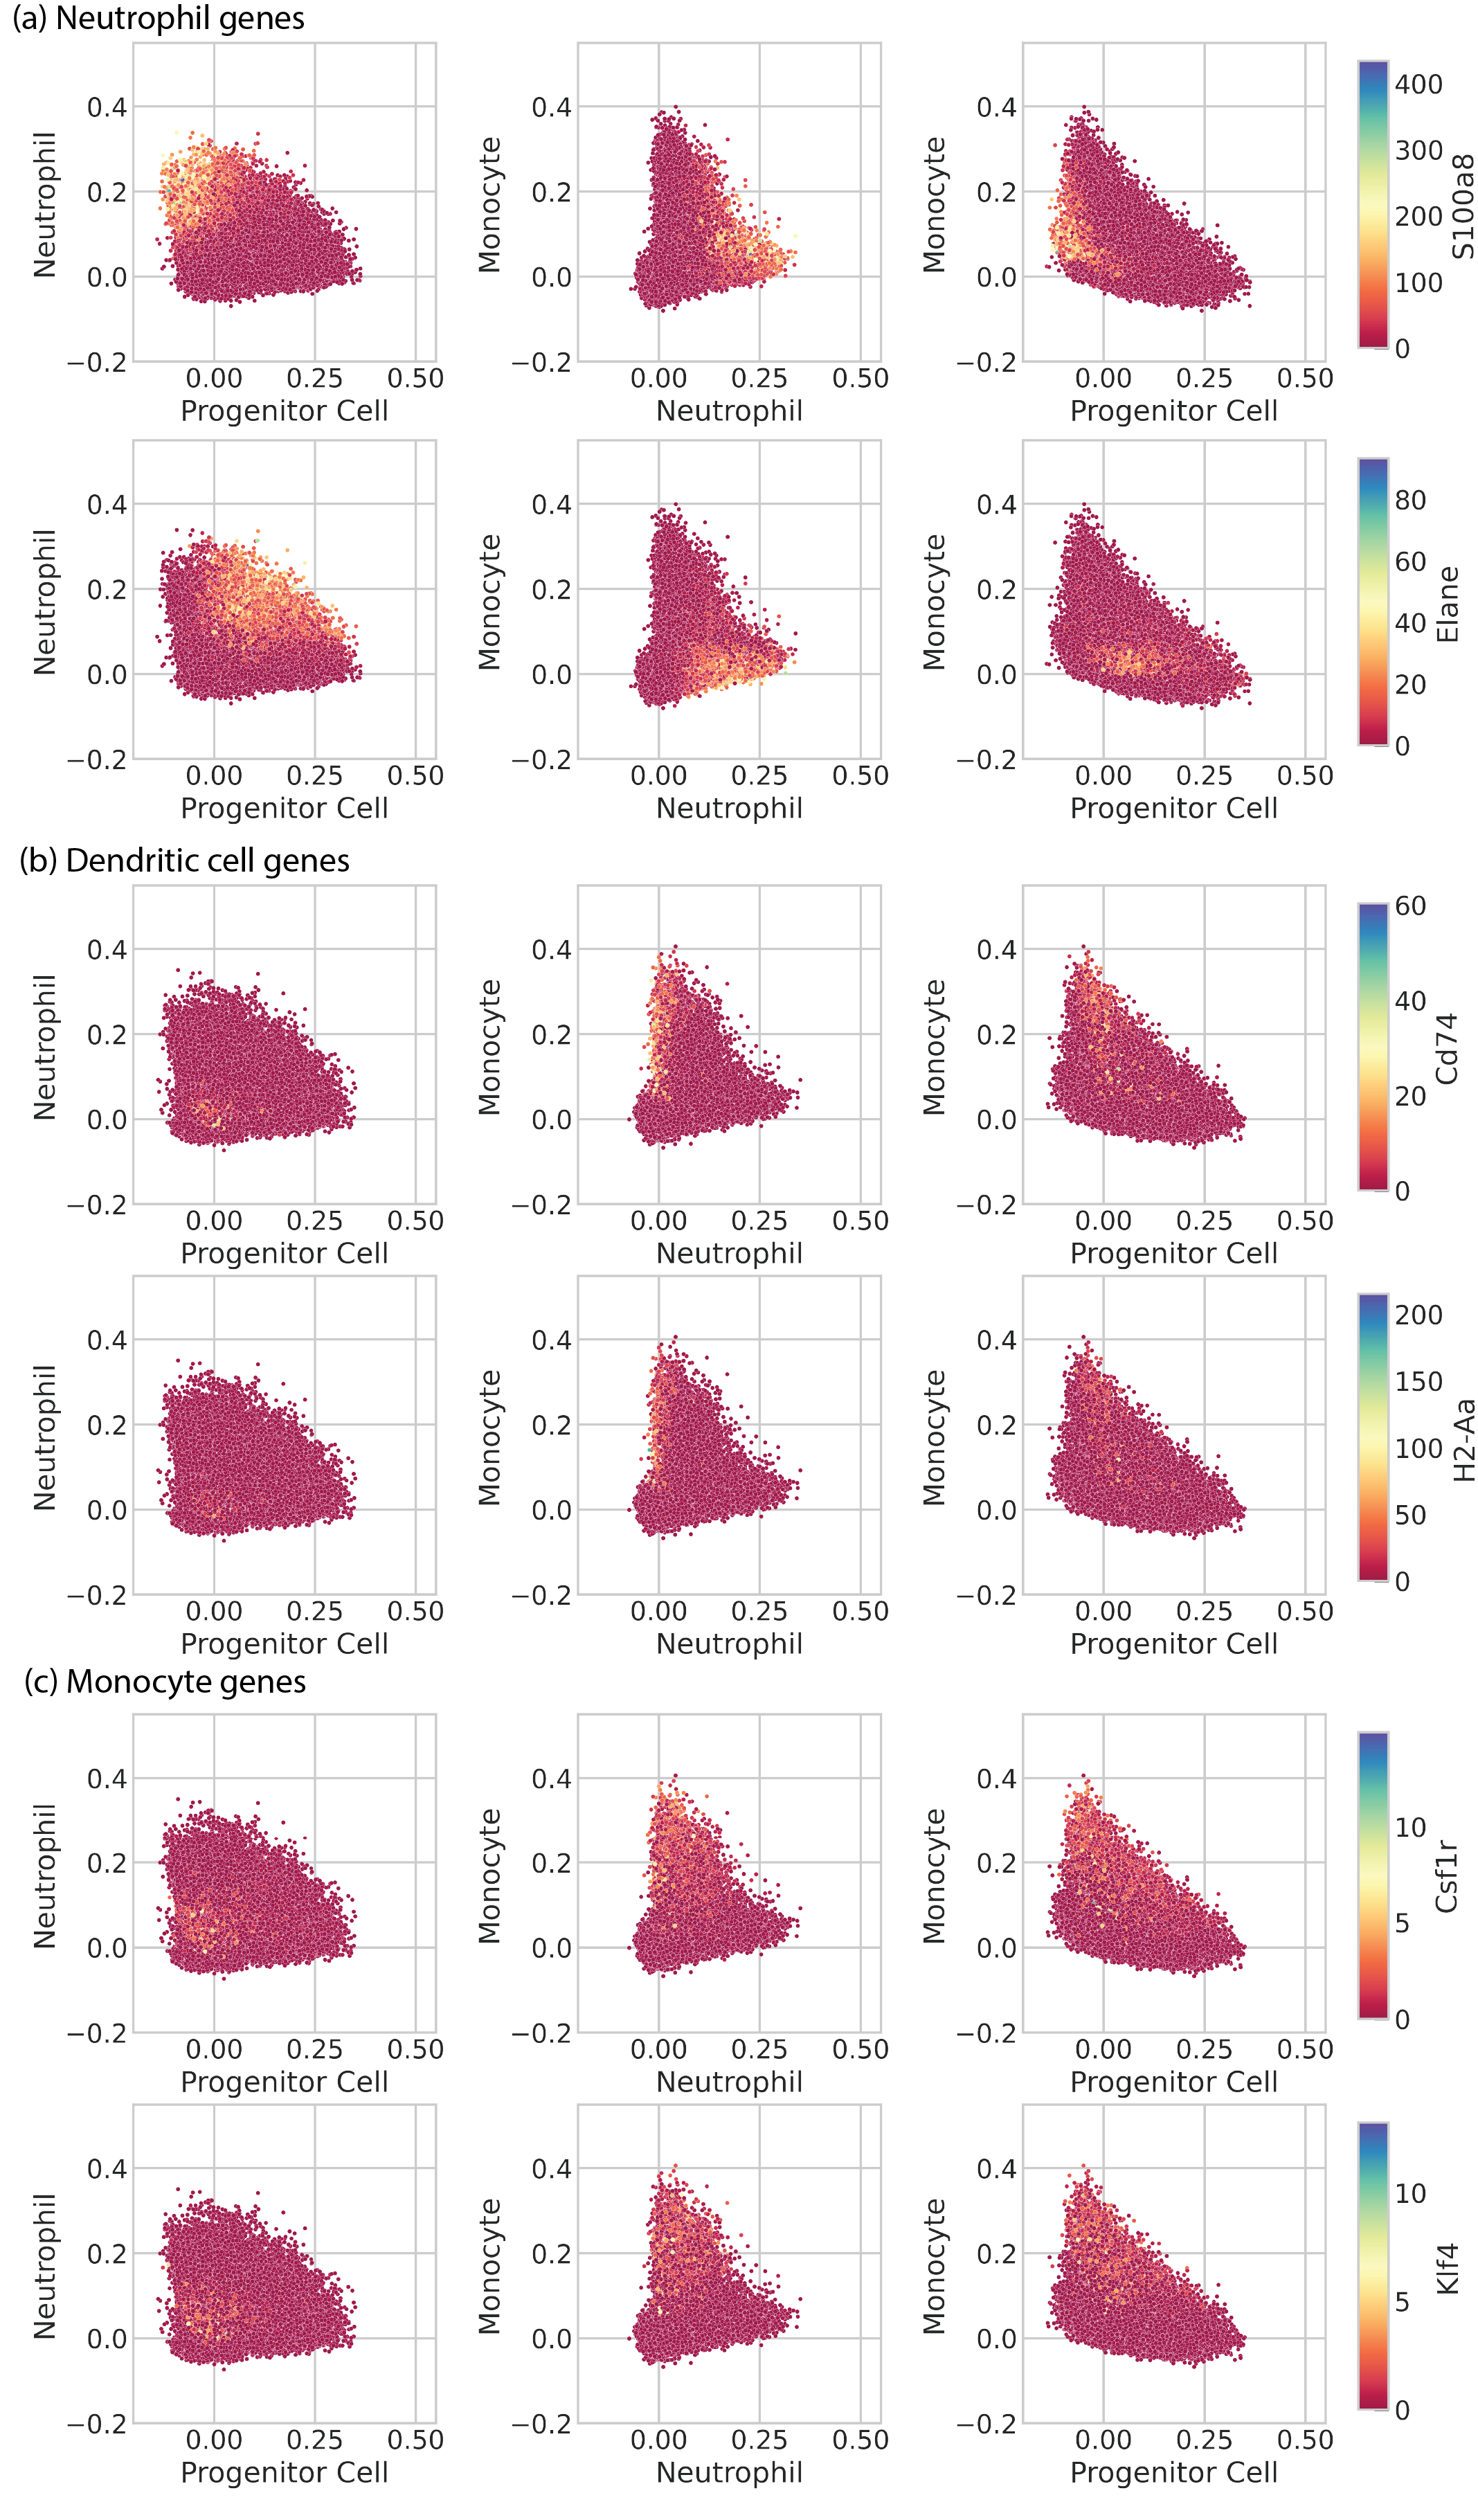
\includegraphics[scale=0.72]{figs/hem genes.png}
	\caption{Scatter plots of in vitro hematopoietic clone families from Weinreb et al., with scTOP scores for progenitor, neutrophil, and monocyte types, and colored by normalized gene expression. In Weinreb et al. figure 4 (a), cells visualized using pseudo-time inference were separated into branches. The monocyte branch appeared to have half of its cells expressing dendritic cell genes and the other half expressing neutrophil genes. This figure plots those same cells on progenitor, neutrophil, and monocyte axes. The colors correspond to neutrophil, dendritic cell, and monocyte marker genes. (a) Hematopoietic cells colored according to the expression of neutrophil marker genes S100a8 and Elane. (b) Hematopoietic cells colored according to the expression of dendritic cell marker genes Cd74 and H2-Aa. (c) Hematopoietic cells colored according to the expression of monocyte marker genes Csf1r and Klf4. }
	\label{hem genes}
\end{figure}

\begin{figure}
	\centering
		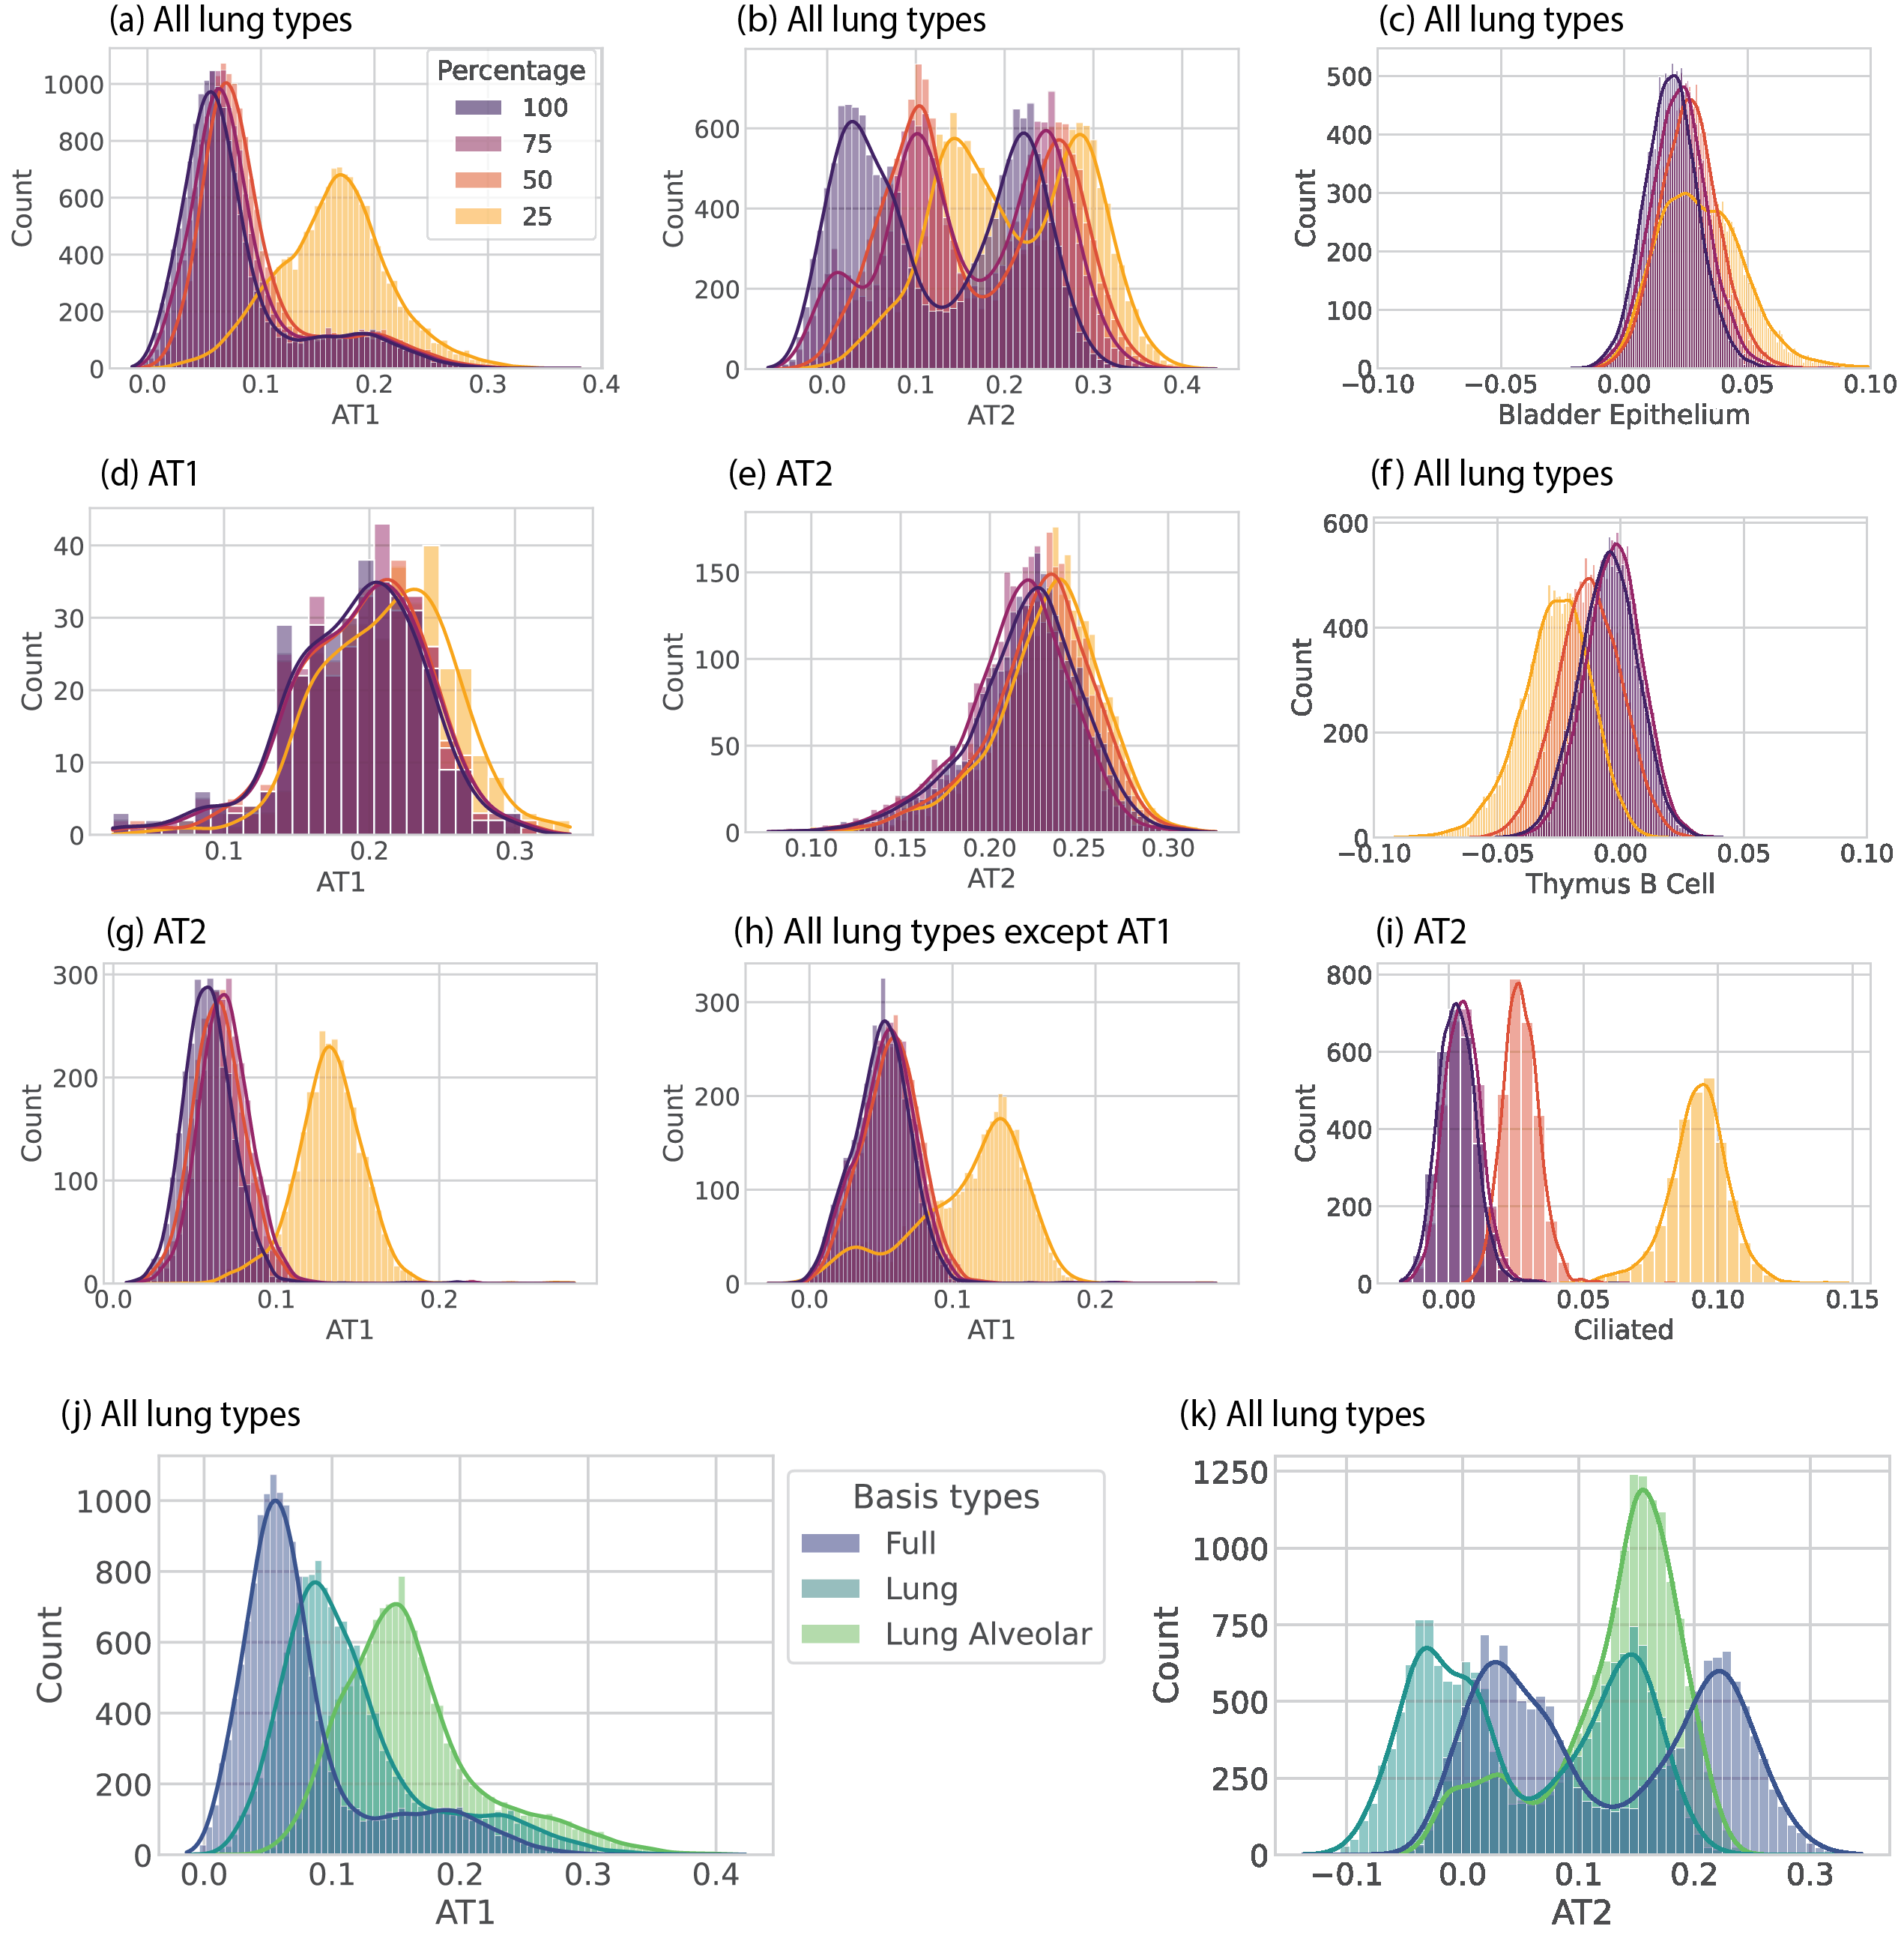
\includegraphics[scale=0.82]{figs/robustness hists.png}
	\caption{Distributions of scTOP scores for lung cells from Herriges et al., using varying portions of the Mouse Cell Atlas as the basis. The label above each plot indicates the Herriges et al. sample subset, while the x-axis label indicates the scTOP reference type. "All lung types" means that all of the lung types from the data set were included. (a) - (i) show how scTOP scores change when 25-100\% of the basis is used. (j) - (k) show how scTOP scores change when the basis is changed from the full basis (which includes many tissues and organs) to just the lung types and to just the two alveolar types. (c) and (f) show scTOP scores for random irrelevant types, Bladder Epithelium and Thymus B Cell, to show that the scTOP scores remain low for types that do not match the sample.}
	\label{robustness hists}
\end{figure}

\subsection{AT1/AT2 marker genes}\label{alveolar markers}
In figure \ref{LungMAP}, plots in (b) and (c) were colored according to AT1 and AT2 marker gene expression. For each cell, the average was taken over the expressions of a set of marker genes. The AT1 marker gene set was:

\begin{itemize}
    \item Ager
    \item Akap5
    \item Aqp5
    \item Cldn18
    \item Clic3
    \item Clic5
    \item Col4a3
    \item Col4a4
    \item Cryab
    \item Cyp2b10
    \item Emp2
    \item Fam189a2
    \item Gprc5a
    \item Hopx
    \item Hs2st1
    \item Igfbp2
    \item Krt7
    \item Lmo7
    \item Mal2
    \item Pdpn
    \item Prdx6
    \item Pxdc1
    \item Rtkn2
    \item Scnn1g
    \item Spock2
    \item Tspan8
    \item Vegfa
\end{itemize}

The AT2 marker gene set was:

\begin{itemize}
    \item Abca3
    \item Acot7
    \item Acoxl
    \item Acsl4
    \item Ank3
    \item Atp8a1
    \item Cd74
    \item Cebpa
    \item Cpm
    \item Ctsh
    \item Cxcl15
    \item Dram1
    \item Egfl6
    \item Elovl1
    \item Etv5
    \item Fabp5
    \item Fasn
    \item Hc
    \item Lamp3
    \item Lgi3
    \item Lpcat1
    \item Lyz2
    \item Mlc1
    \item Muc1
    \item Napsa
    \item Npc2
    \item Ppp1r14c
    \item S100g
    \item Scd1
    \item Sfta2
    \item Sftpa1
    \item Sftpb
    \item Sftpc
    \item Sftpd
    \item Slc34a2
    \item Zdhhc3
\end{itemize}

\begin{figure}
	\centering
	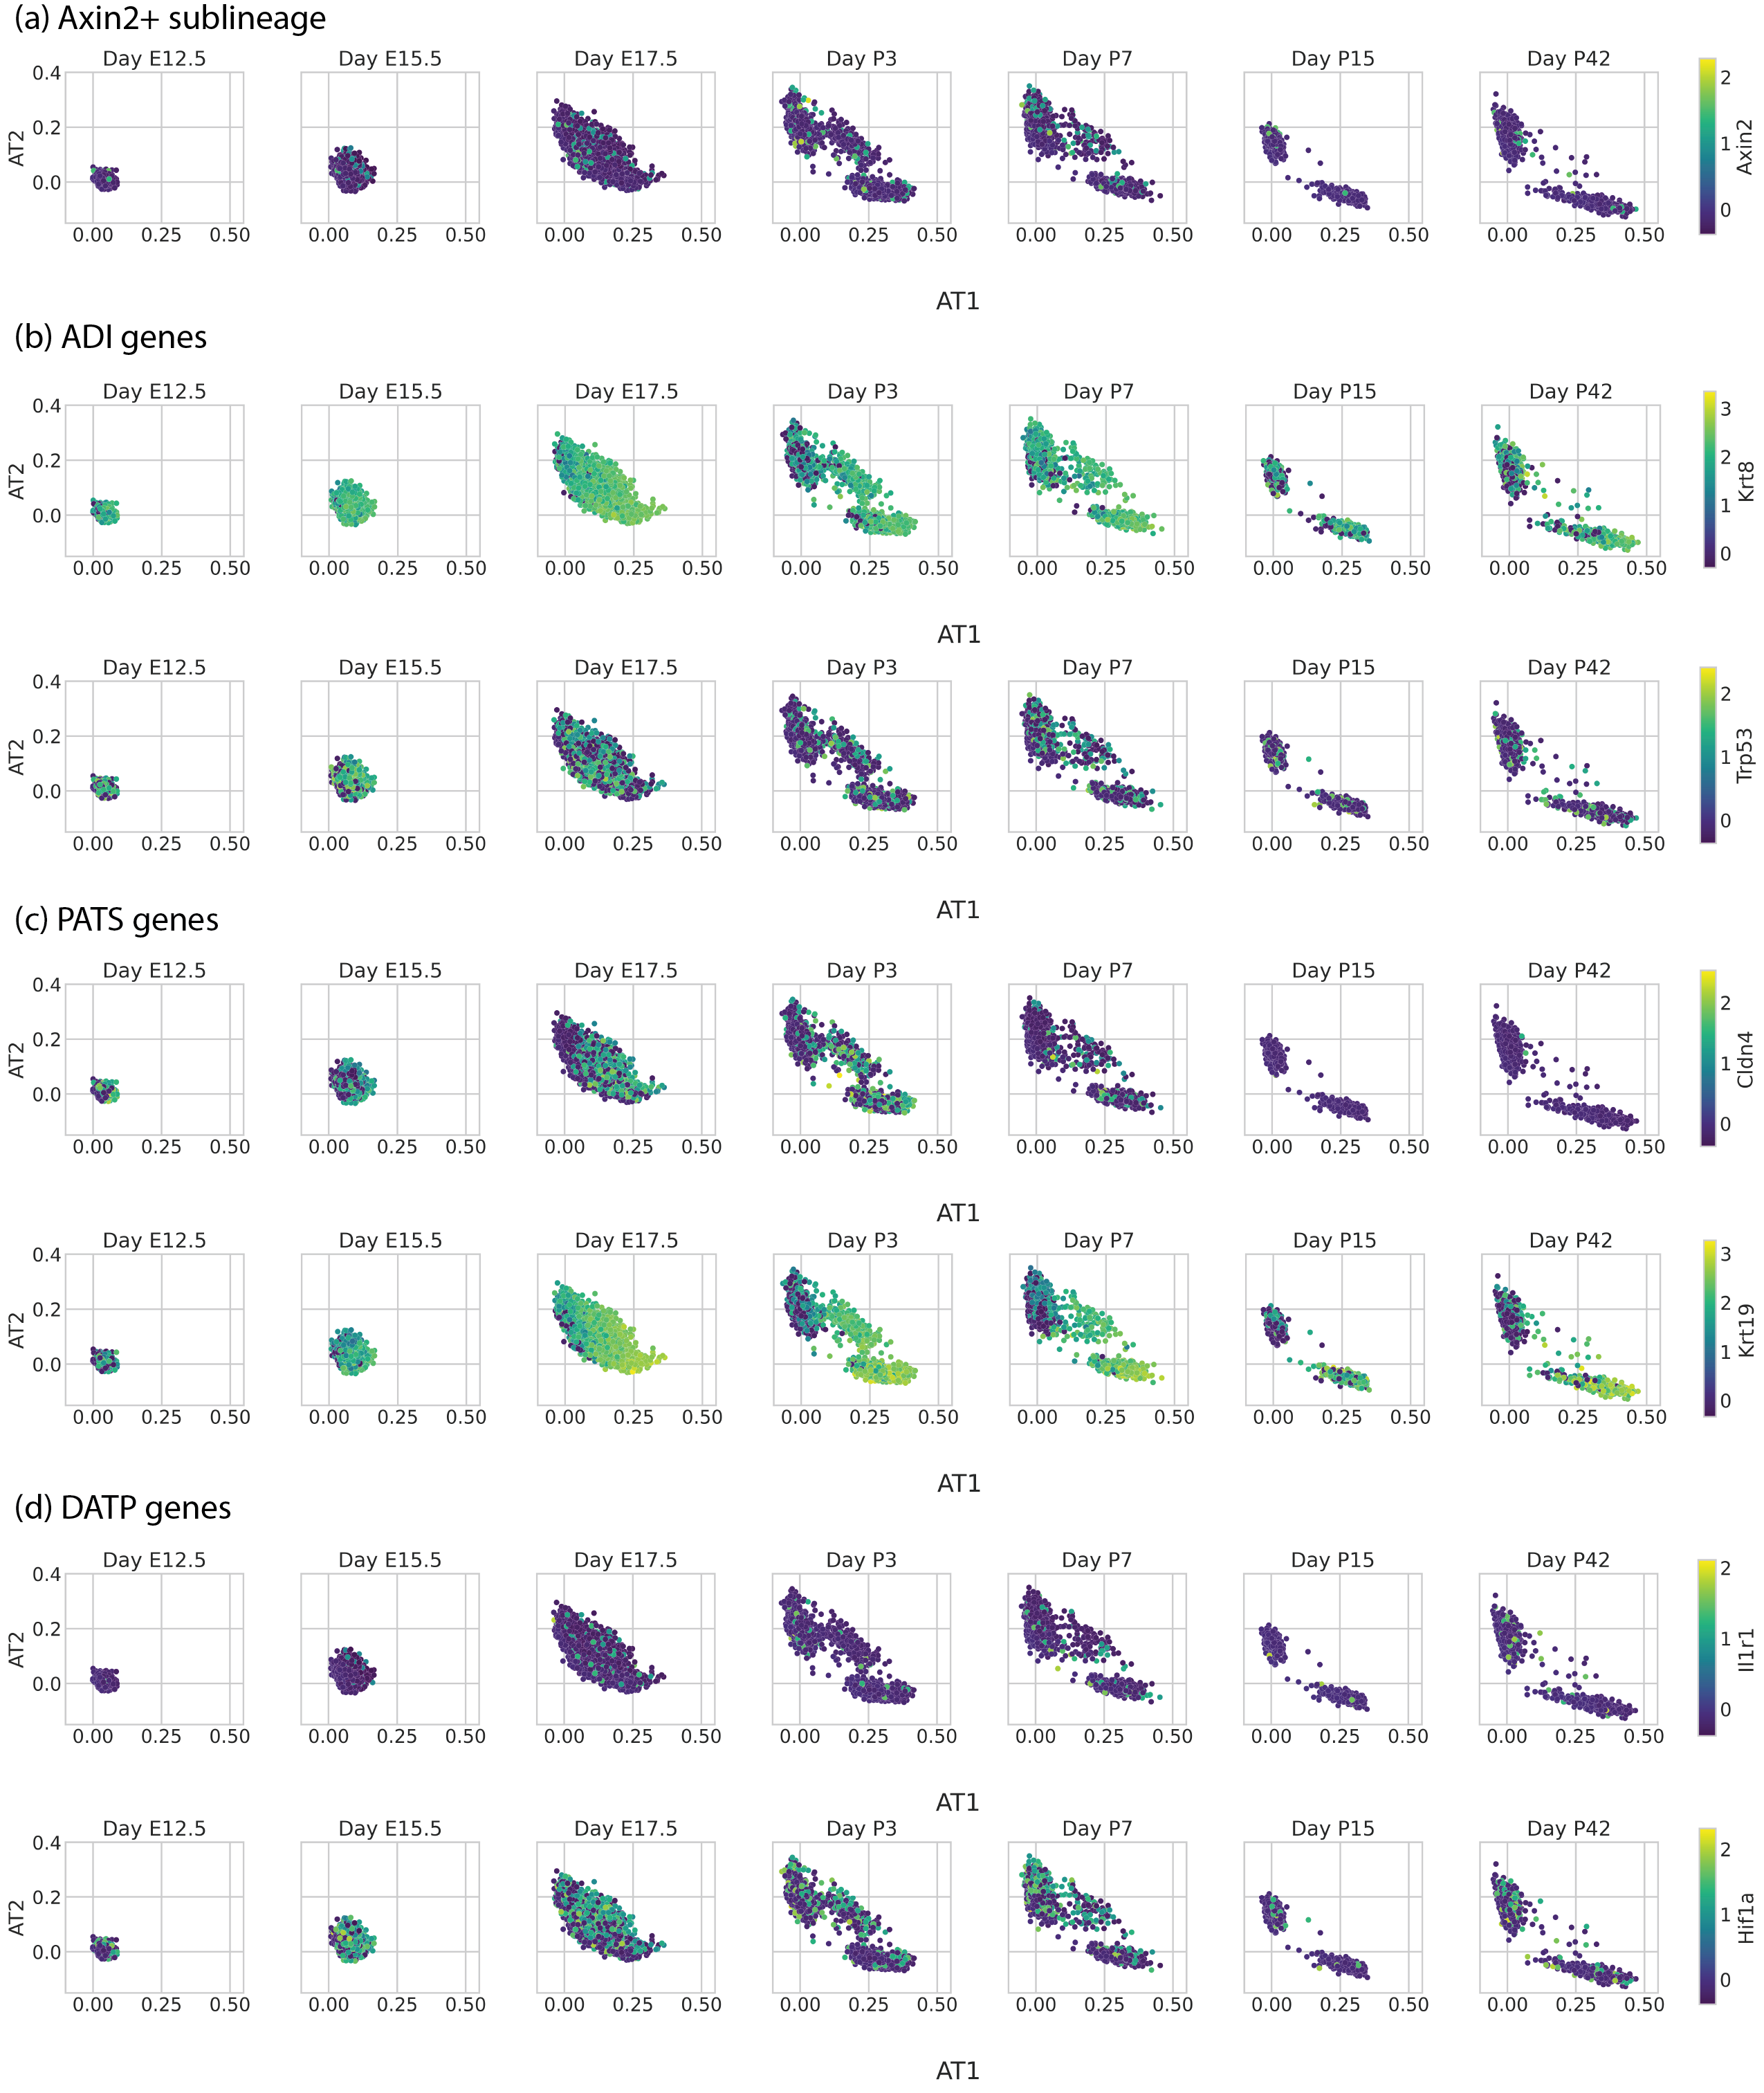
\includegraphics[scale=0.8]{figs/LungMAP genes.png}
	\caption{The AT1/AT2 combination state (most apparent in days P3 and P7) do not uniquely express genes of AT1/AT2 transitional states described by previous papers. Alveolar cells from Zepp et al. are plotted on AT1 and AT2 axes, separated by day. Each cell is colored by the expression z-score of a particular gene, and the particular gene is different in each row. The gene used to color the cells is indicated by the color bar on the far right of each row. (a) Alveolar cells colored by Axin2, showing that the AT1/AT2 combination cells do not appear to belong to the Axin2+ sublineage described by  \cite{frank2016emergence}. (b) Alveolar cells colored by Krt8 and Trp53 expression, which are genes corresponding to alveolar differentiation intermediate cells (ADI) described by \cite{strunz2020alveolar}. AT1, AT2, and the combination AT1/AT2 state all express Krt8 and Trp53 at similar levels. (c) Alveolar cells colored by expression of pre-alveolar type-1 transitional cell state (PATS) genes described by \cite{kobayashi2020persistence}. AT1, AT2, and the combination AT1/AT2 state all express Cldn4 at similar levels. AT1 and AT1/AT2 combination cells both express Krt19 at similar levels, although AT1 cells express the gene at higher levels. (d) Alveolar cells colored by expression of damage-associated transient progenitor (DATP) genes described by \cite{choi2020inflammatory}. AT1, AT2, and the combination AT1/AT2 state all express Il1r1 and HIF1a at similar levels. }
	\label{LungMAP genes}
\end{figure}

\begin{figure}
	\centering
	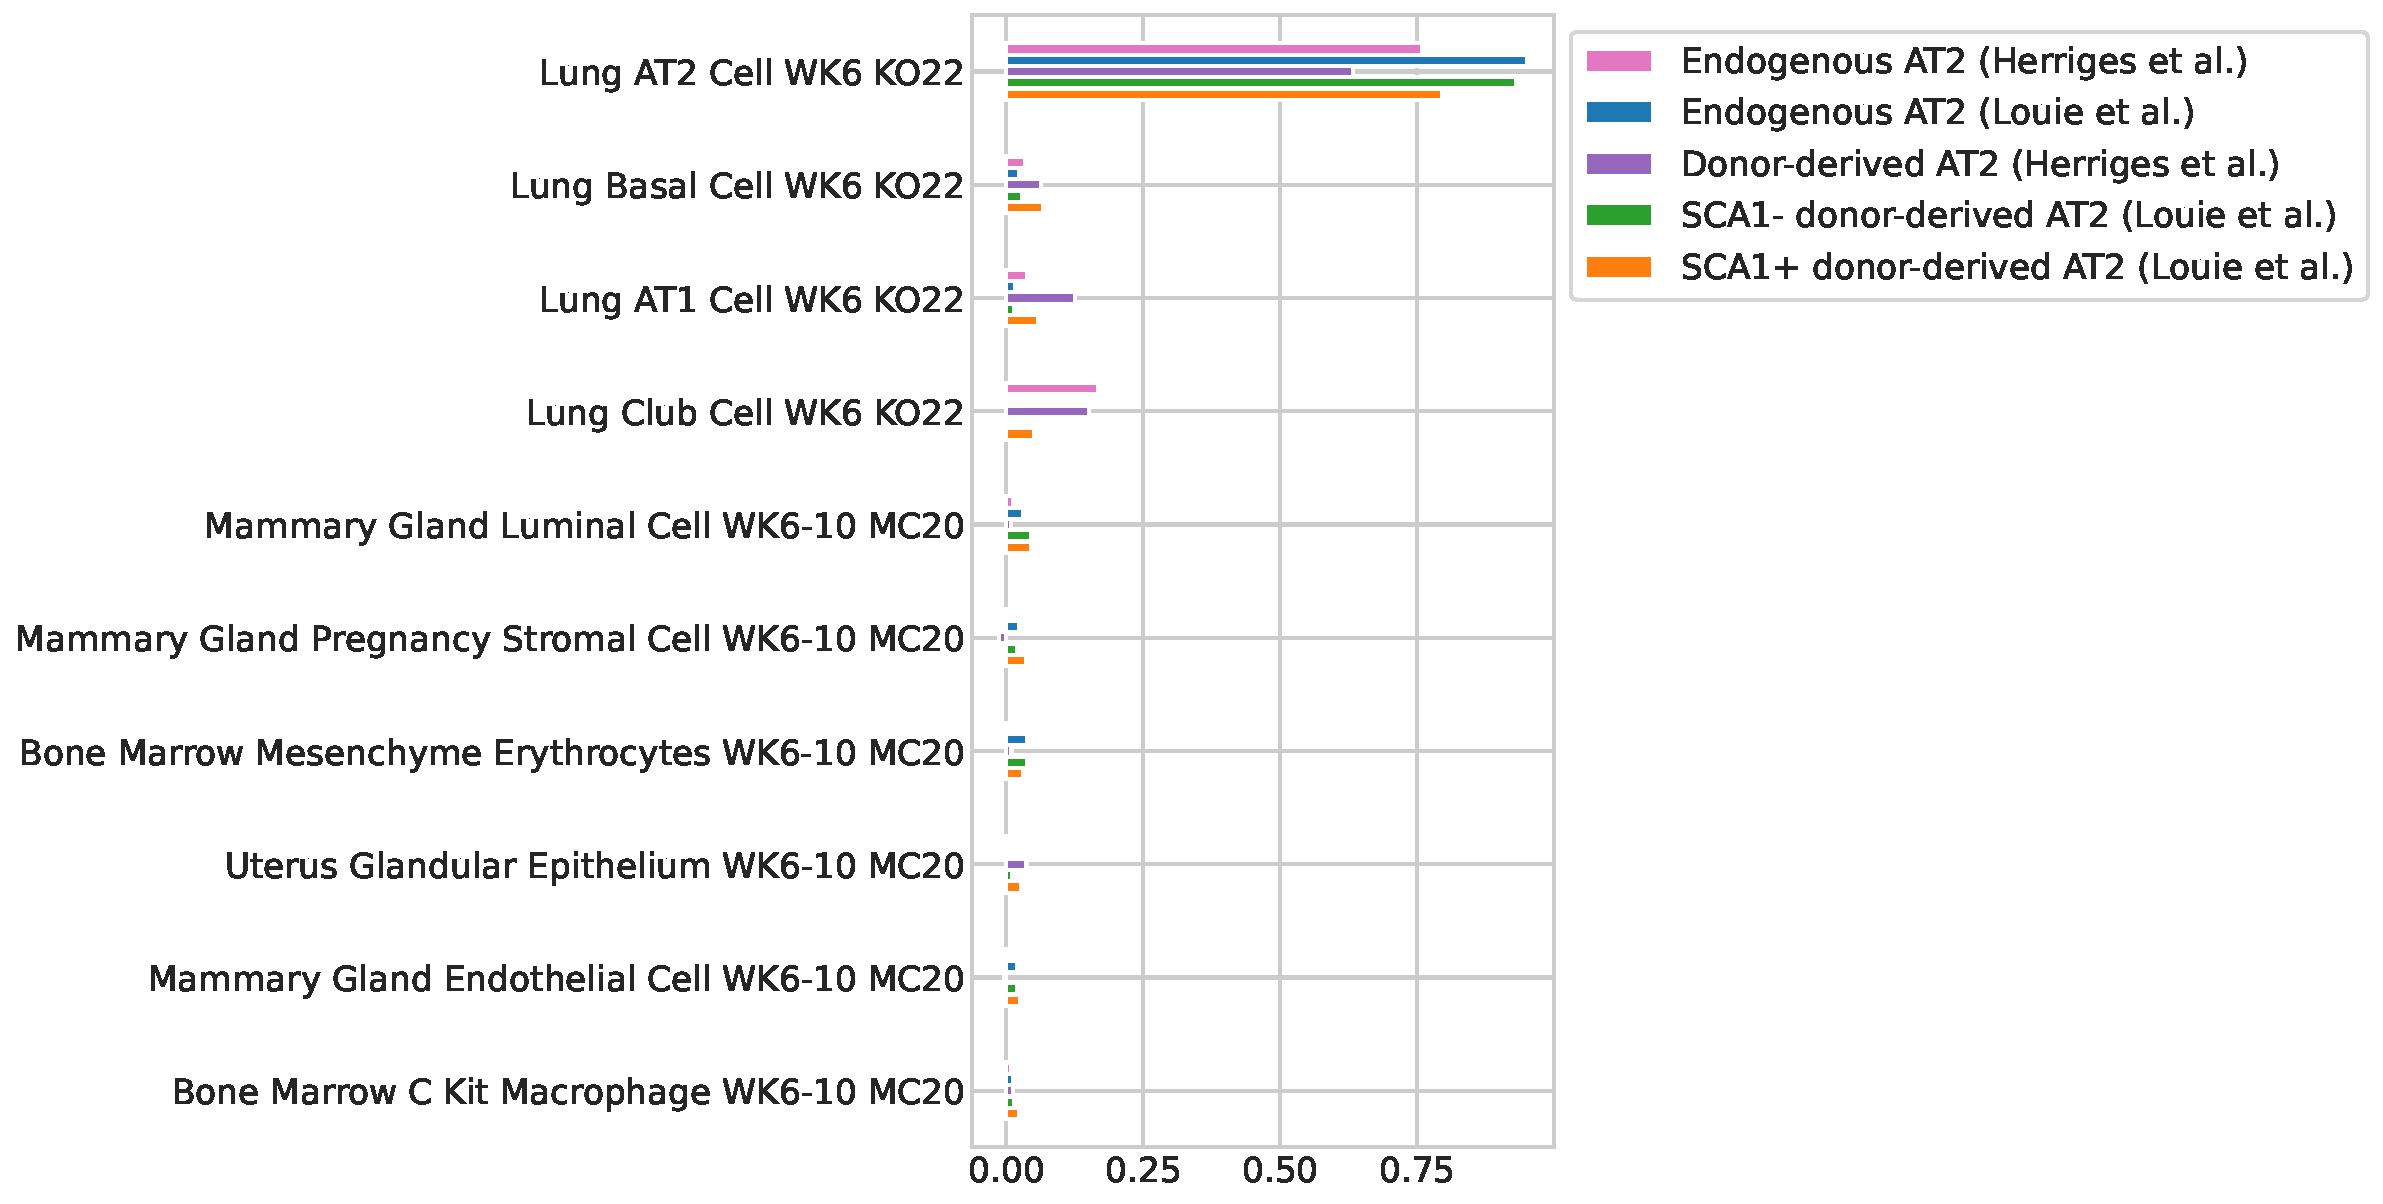
\includegraphics[scale=0.4]{figs/lung barplot.pdf}
	\caption{Bar plot showing the top ten aggregate scores for the AT2 populations from the various endogenous and transplanted sources shown in Figure 9 of the main text. The cell types are ranked according to the magnitude of scores for the SCA1+ population.}
    \label{barplot}
\end{figure}

\bibliography{export-data.bib}

\end{document}